\documentclass[unknownkeysallowed]{beamer}
\usepackage[french,english]{babel}
\usepackage{../sty/beamer_js}
\usepackage{../sty/shortcuts_js}


\begin{document}


%%%%%%%%%%%%%%%%%%%%%%%%%%%%%%%%%%%%%%%%%%%%%%%%%%%%%%%%%%%%%%%%%%%%%%%%%%%%%%%
%%%%%%%%%%%%%%%%%%%%%%             Headers               %%%%%%%%%%%%%%%%%%%%%%
%%%%%%%%%%%%%%%%%%%%%%%%%%%%%%%%%%%%%%%%%%%%%%%%%%%%%%%%%%%%%%%%%%%%%%%%%%%%%%%



%%%%%%%%%%%%%%%%%%%%%%%%%%%%%%%%%%%%%%%%%%%%%%%%%%%%%%%%%%%%%%%%%%%%%%%%%%%%%%%
\begin{frame}
\bigskip
\bigskip
\begin{center}{
\LARGE\color{marron}
\textbf{Outlier-robust estimation of a sparse linear model using l1-penalized Huber's M-estimator}
\textbf{ }\\
\vspace{0.5cm}
}

\color{marron}
\textbf{}
\end{center}

\vspace{0.5cm}

\begin{center}
\textbf{Rudolf Römisch} \\
\vspace{0.5cm}
Université de Montpellier \\
\end{center}

\centering
\includegraphics[width=0.13\textwidth]{Logo}

\end{frame}
%%%%%%%%%%%%%%%%%%%%%%%%%%%%%%%%%%%%%%%%%%%%%%%%%%%%%%%%%%%%%%%%%%%%%%%%%%%%%%%



%%%%%%%%%%%%%%%%%%%%%%%%%%%%%%%%%%%%%%%%%%%%%%%%%%%%%%%%%%%%%%%%%%%%%%%%%%%%%%%
%%%%%%%%%%%%%%%%%%%%%%%%       PLAN      %%%%%%%%%%%%%%%%%%%%%%%%%%%%%%%%%%%%%%
%%%%%%%%%%%%%%%%%%%%%%%%%%%%%%%%%%%%%%%%%%%%%%%%%%%%%%%%%%%%%%%%%%%%%%%%%%%%%%%



%%%%%%%%%%%%%%%%%%%%%%%%%%%%%%%%%%%%%%%%%%%%%%%%%%%%%%%%%%%%%%%%%%%%%%%%%%%%%%%
\begin{frame}{Table of Contents}
\tableofcontents[hideallsubsections]
\end{frame}
%%%%%%%%%%%%%%%%%%%%%%%%%%%%%%%%%%%%%%%%%%%%%%%%%%%%%%%%%%%%%%%%%%%%%%%%%%%%%%%



%%%%%%%%%%%%%%%%%%%%%%%%%%%%%%%%%%%%%%%%%%%%%%%%%%%%%%%%%%%%%%%%%%%%%%%%%%%%%%%
\AtBeginSection[]
{
\begin{frame}<beamer>{Table of Contents}
\tableofcontents[currentsubsection,
    hideothersubsections,
    sectionstyle=show/shaded,
]
\end{frame}
}
%%%%%%%%%%%%%%%%%%%%%%%%%%%%%%%%%%%%%%%%%%%%%%%%%%%%%%%%%%%%%%%%%%%%%%%%%%%%%%%




%%%%%%%%%%%%%%%%%%%%%%%%%%%%%%%%%%%%%%%%%%%%%%%%%%%%%%%%%%%%%%%%%%%%%%%%%%%%%%%
%%%%%%%%%%%%%%%%%%%%%%%%%%%%%%%%%%%%%%%%%%%%%%%%%%%%%%%%%%%%%%%%%%%%%%%%%%%%%%%
\section{Introduction}
\label{sec:introdcution}
%%%%%%%%%%%%%%%%%%%%%%%%%%%%%%%%%%%%%%%%%%%%%%%%%%%%%%%%%%%%%%%%%%%%%%%%%%%%%%
%%%%%%%%%%%%%%%%%%%%%%%%%%%%%%%%%%%%%%%%%%%%%%%%%%%%%%%%%%%%%%%%%%%%%%%%%%%%%%%

%%%%%%%%%%%%%%%%%%%%%%%%%%%%%%%%%%%%%%%%%%%%%%%%%%%%%%%%%%%%%%%%%%%%%%%%%%%%%%%
\label{sub:un_premier_exemple}
%%%%%%%%%%%%%%%%%%%%%%%%%%%%%%%%%%%%%%%%%%%%%%%%%%%%%%%%%%%%%%%%%%%%%%%%%%%%%%%

%%%%%%%%%%%%%%%%%%%%%%%%%%%%%%%%%%%%%%%%%%%%%%%%%%%%%%%%%%%%%%%%%%%%%%%%%%%%%%%

\begin{frame}{Introduction}
	\begin{itemize}
		\item Optimal rates of estimation in outlier-robust sparse regression using penalized empirical risk minimization (PERM) with convex loss and convex penalties?
		\item Current state of literature,
		\item Assumptions and resulting setting.
	\end{itemize}
\end{frame}

\begin{frame}{Basic Model}
	Let $\mathcal{D}_n$° = $\{(\boldmath{X}_i, y_i$°$); i = 1,...,n \}$ be the independed identical distributed (i.i.d.) feature-label pairs.\\
	\begin{equation*}
	y_i^{\circ} = \bold{X}_i^T\beta^* + \xi_i, \quad i=1,...,n
	\end{equation*}
	
	\begin{itemize}
		\item  $\boldmath{X}_i \in \mathbb{R}^p$ are Gaussian with zero mean and covariance matrix $\Sigma$,
		\item  $y_i^{\circ}$ are the responses defined by the linear model above,
		\item  $\xi_i $~$ \mathcal{N}(0,\sigma^2)$ is the random noise which is independent of $\boldmath{X}_i$
	\end{itemize}
\end{frame}



\begin{frame}{Contaminated Model}
	
	\begin{equation*}
	\bold{Y} = \bold{X\beta^*} + \sqrt{n} \boldsymbol{\theta^*} + \boldsymbol{\xi},
	\end{equation*}
	
	\begin{itemize}
		\item $\boldmath{X} = [\boldmath{X}_1^T;...;\boldmath{X}^T_n]$ is the $n\times p$ design matrix,
		\item $\boldmath{Y}$ = $(y_1,...,y_n)^T$ is the response vector,
		\item $ \boldsymbol{\theta^*} = (\theta^*_1,...,\theta^*_n)^T$ is the contamination with $\theta^*_i = (y_i - y_i^{\circ})/\sqrt{n}$,
		\item $\boldsymbol{\xi} = (\xi_1,...,\xi_n)^T$ is the noise vector.
	\end{itemize}
	In the following, it is the goal to estimate the vector $\boldsymbol{\beta}^* \in \mathbb{R}^p$.
\end{frame}



\begin{frame}{$l_1$-penalized ERM}
	
	\begin{equation*}
	\hat{\bold{\beta}} \in arg
	\min\limits_{\bold{\beta}\in
		\mathbb{R}^p} \min\limits_{\bold{\theta}\in
		\mathbb{R}^n}\{\frac{1}{2n} ||\bold{Y} - \bold{X^T\beta} - \sqrt{n}\bold{\theta}||_2^2 + \lambda_s ||\bold{\beta}||_1 + \lambda_o||\bold{\theta}||_1\}
	\end{equation*}
	
\end{frame}


\begin{frame}{$l_1$-penalized Huber's M-estimator}
	\begin{equation*}
	\hat{\beta} \in arg \min\limits_{\bold{\beta}\in
		\mathbb{R}^p} \{ \lambda_o^2 \sum_{i = 1}^{n}\Phi (\frac{y_i - \bold{X}^T_i \bold{\beta}}{\lambda_o \sqrt{n}}) + \lambda_s||\bold{\beta}||_1\}
	\end{equation*}
\end{frame}



\section{Risk Bound}

\begin{frame}{Restricted Invertibility and Incoherence}
	\begin{definition}
		Let $ \bold{Z} \in \mathbb{R}^{nxp} $ be a (random) matrix and $ \Sigma \in \mathbb{R}^{pxp} $. We use notation $ \bold{Z}^{(n)} = \bold{Z}/\sqrt{n}$.\\
		\begin{itemize}
			\item (i) We say that $\bold{Z}$ satisfies the transfer principle with $a_1 \in (0,1)$ and $a_2 \in (0,\infty)$, denoted by $TP_{\Sigma}(a_1;a_2)$, if for all $\bold{v} \in \mathbb{R}^p$,
			\begin{equation}
			||\bold{Z}^{(n)}||_2 \geq a_1 ||\Sigma^{1/2}\bold{v}||_2 - a_2||\bold{v}||_1
			\end{equation}
			
			\item (ii) We say that $\bold{Z}$ satisfies the incoherence property $IP_{\Sigma}(b_1;b_2;b_3)$ for some positive numbers $b_1, b_2 and b_3$, if for all $[v;u] \in \mathbb{R}^{p+n}$,
			\begin{equation}
			|u^T Z^{(n)}v| \leq b_1||\Sigma^{1/2}v||_2||u||_2 + b_2||v||_1||u||_2 + b_3||\Sigma^{1/2}v||_2||u||_1.
			\end{equation}
			\item (iii) We say that $ \bold{Z} $ satisfies the augmented transfer principle $ATP_{\Sigma}(c_1;c_2;c_3)$ for some positive numbers $c_1, c_2 and c_3$, if for all $[v;u]\in \mathbb{R}^{p+n}$,
			\begin{equation}
			||\bold{Z}^{(n)}v+u||_2 \geq c_1||[\Sigma^{1/2}v;u]||_2 - c_2||v||_1 - c_3||u||_1.
			\end{equation}
		\end{itemize}
	\end{definition}
\end{frame}


\begin{frame}{Bound Theorem}
	Prerequisites:\\
	1. We assume $\lambda_s = \lambda_o = \lambda$\\
	2. Normalization of the columns of the matrix $\boldmath{X}$, so that their Euclidean nor is of the order $\sqrt{n}$\\
	3. A matrix $\Sigma$ is said to satisfy the restricted eigenvalue condition $RE(s,c_0)$ with some constant $\varkappa >0$, if
	\begin{equation*}
	||\Sigma^{1/2}\bold{v}|| \geq \varkappa ||\bold{v}_J||_2
	\end{equation*}
	for any vector $\bold{v}\in \mathbb{R}^p$ and any set $J \subset \{1,...,p\}$ such that $Card(J) = \leq s$ and $||\bold{v}_{J^c}||_1 \leq c_0||\bold{v}_J||_1$.
	
\end{frame}



\begin{frame}{Main Theorem}
	\begin{theorem}\ \\
		Let $\Sigma$ satisfy the RE(s,5) condition with constant $\varkappa > 0$. Let $b_1,b_2,b_3, c_1, c_2, c_3$ be some positive real numbers such that $\bold{X}$ satisfies the $IP_{\Sigma}(0;b_2;b_3)$ and the $ATP_{\Sigma}(c_1;c_2;c_3)$. Assume that for some $\delta \in (0,1)$, the tuning parameter $\lambda$ satisfies
		\begin{equation*}
		\lambda \sqrt{n} \leq \sqrt{8 log(n/\delta)} \bigvee (\max\limits_{j = 1,...,p}||\bold{X}_{\bullet, j}^{(n)}||_2)\sqrt{8log(p/\delta)}.
		\end{equation*}
		If the sparsity s and the number of outliers o satisfy the condition
		\begin{equation*}
		\frac{s}{\varkappa^2} + o \leq \frac{c_1^2}{400(c_2 \vee c_3 \vee 5b_2/c_1)},
		\end{equation*}
		then, with probability at least $1-2\delta$, we have
		\begin{equation*}
		||\bold{\Sigma}^{1/2}(\hat{\beta}- \beta^*)||_2 \leq \frac{24\lambda}{c_1^2}(\frac{2c_2}{
			c_1} \bigvee \frac{b_3}{c_1^2}) (\frac{s}{\varkappa^2} + 7o) + \frac{5\lambda\sqrt{s}}{6c_1^2\varkappa}.
		\end{equation*}
	\end{theorem}
\end{frame}


\section{Gaussian Design}

\begin{frame}{}
	\begin{theorem}\ \\
		There exist universal positive constants $d_1, d_2, d_3$ such that if
		\begin{equation}
		\frac{s log(p)}{\varkappa^2} + o log(n) \leq d_1n \quad and \quad 1/7 \geq \delta \geq 2e^{-d_2n}
		\end{equation}
		then, with probability at least $1-4\delta$, $l_1$-penalized Huber's M-estimator with $\lambda^2_sn = 9\sigma^2 log (p/\delta)$ and $\lambda^2_on = 8\sigma^2 log (n/\delta)$ satisfies
		\begin{equation*}
		||\bold{\Sigma}^{1/2}(\hat{\beta}-\beta^*)||_2 \leq d_3 \sigma \Big\{ (\frac{slog(p/\delta)}{n\varkappa^2})^{1/2} + \frac{olog(n/\delta)}{n} \Big\}.
		\end{equation*}
	\end{theorem}

\end{frame}


\section{Extensions}
\begin{frame}{Extensions}
	\begin{itemize}
		\item Contaminated Design
		\item Sub-Gaussian Design
		\item Heavier tailed Noise Distribution
	\end{itemize}
\end{frame}


\section{Numerical Illustration}


\begin{frame}
	\begin{center}
		\centering
		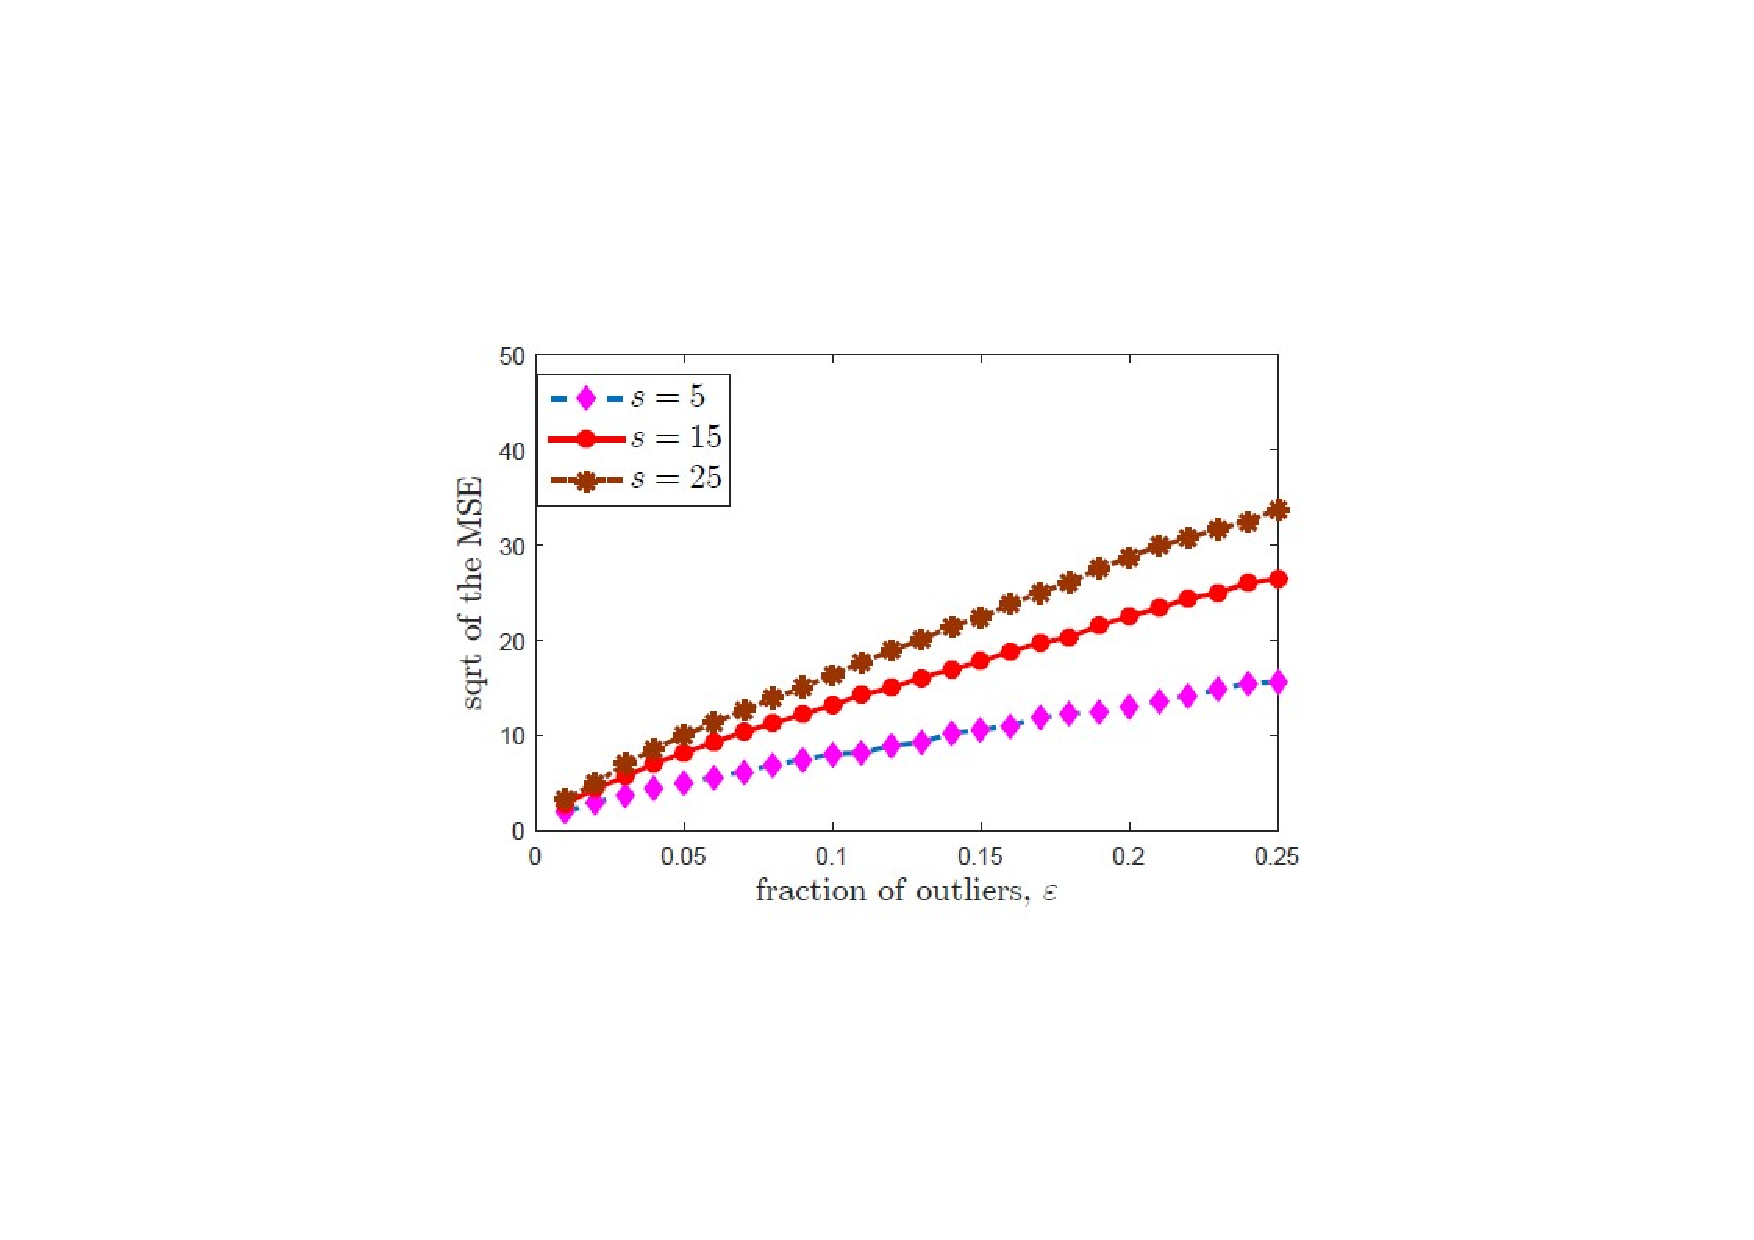
\includegraphics{numerical_illustration.pdf}
	\end{center}
	
\end{frame}




%%%%%%%%%%%%%%%%%%%%%%%%%%%%%%%%%%%%%%%%%%%%%%%%%%%%%%%%%%%%%%%%%%%%%%%%%%%%%%%






\end{document}
